\chapter{Manual de utilizare}

\section{Pașii de utilizare}
Pentru utilizarea aplicației {\applicationtitle}, utilizatorul va urma pașii:
\begin{enumerate}
    \item Va apasă butonul de "Login" de pa pagina principală
    \item Se va autentifica în contul de Flickr, pe pagina de Flickr pe care a fost redirectat
    \item Va autoriza accesul aplicației la contul său de Flickr, apăsând "Authorize" din pagina deschisă de Flickr
    \item Va apăsa butonul de "Choose file", apoi va alege o imagine de pe propriul dispozitiv
    \item Va alege una din opțiunile sursei imaginilor ce vor fi analizate, apăsând unul din cele trei \textit{radio-buttons} disponibile
    \item Va apăsa butonul "Upload"
    \item Aplicația îi va procesa cererea, apoi va afișa etichetele corespunzătoare imaginii și imaginile similare vizual, sau mesaje explicative dacă nu au fost găsite etichete/imagini corespunzătoare
\end{enumerate}{}

Procesul de utilizare  este simplificat de faptul că nu există nevoia de crearea de credențiale separate pentru aplicație, ci se folosește direct rutina de autentificare a platformei Flickr. 

\section{Scenariu de utilizare}
\subsection{Utilizatorul accesează pagina principală}

\begin{figure}[!htbp]
    \begin{center}
        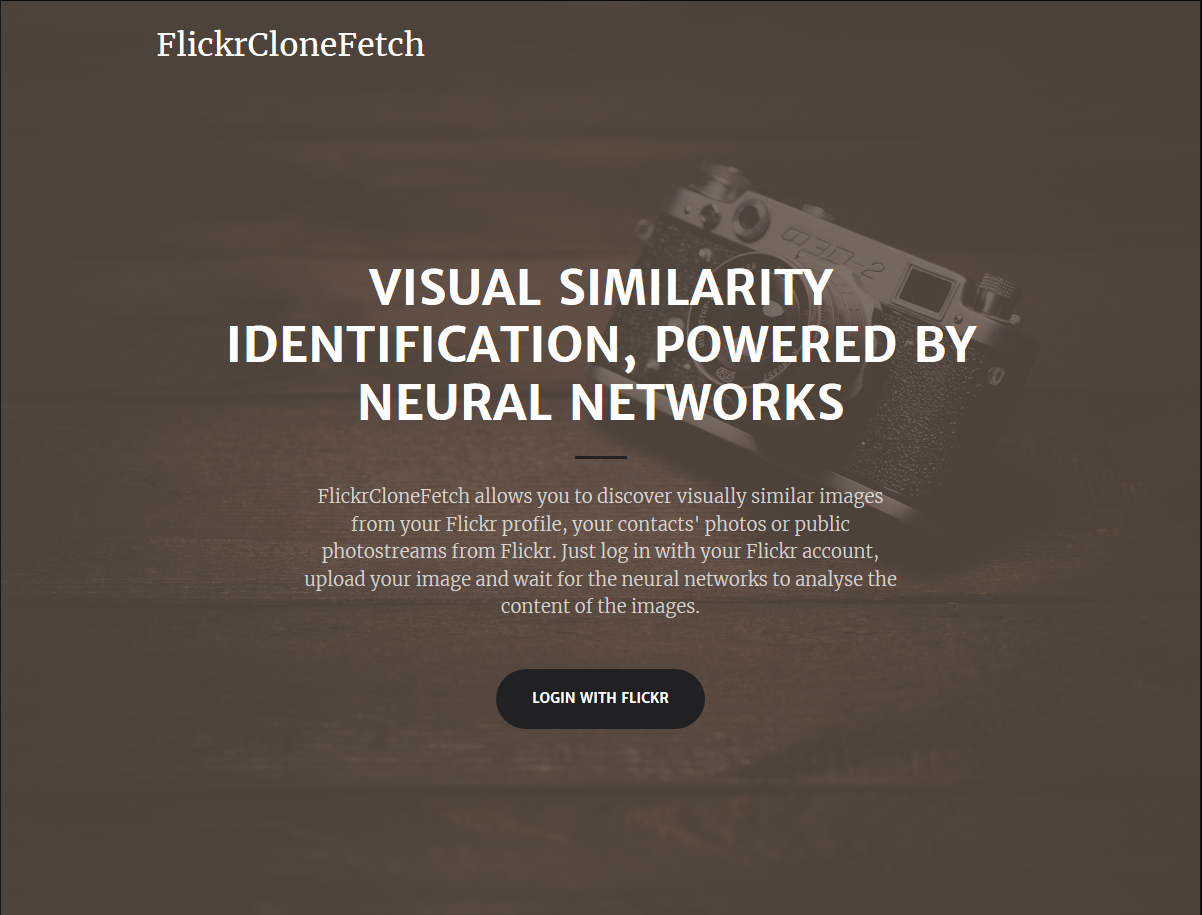
\includegraphics[width=1.0\textwidth]{images/home_page.png}
        \caption{Pagina principală }
    \end{center}
\end{figure}

\pagebreak
\subsection{Utilizatorul autorizează aplicația}

\begin{figure}[!htbp]
    \begin{center}
        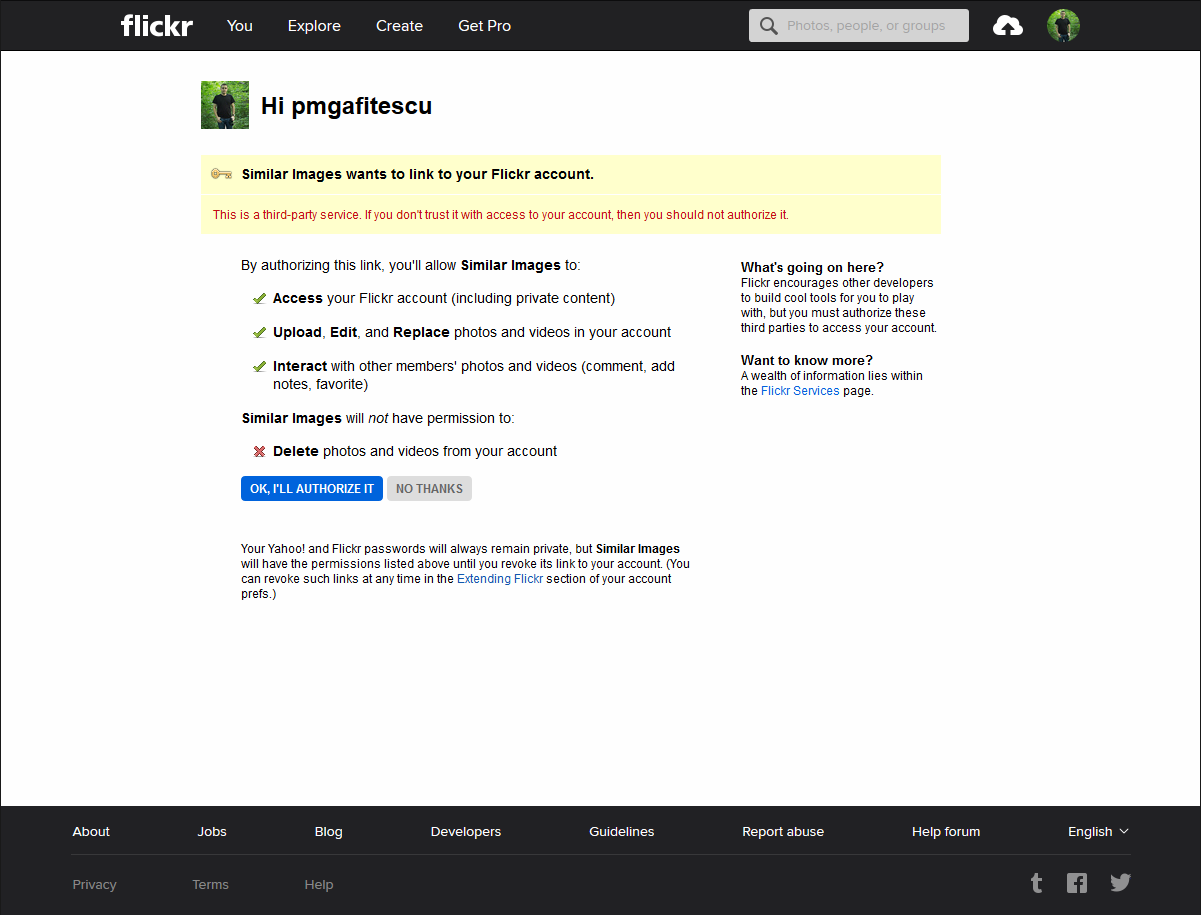
\includegraphics[width=1.0\textwidth]{images/authorize.png}
        \caption{Autorizarea aplicației }
    \end{center}
\end{figure}


\pagebreak
\subsection{Pagina de încărcare a unei imagini}

\begin{figure}[!htbp]
    \begin{center}
        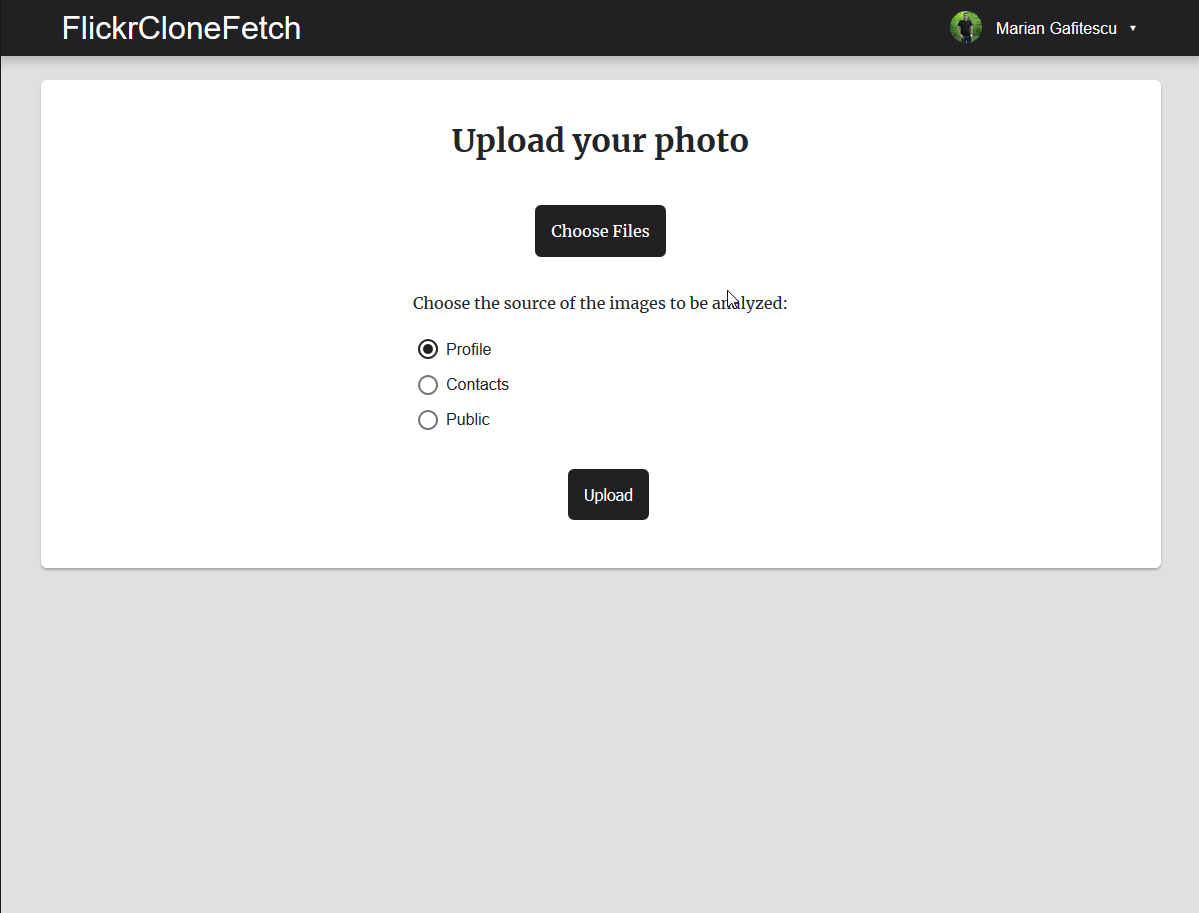
\includegraphics[width=1.0\textwidth]{images/choose.png}
        \caption{Pagina de încărcare a unei imagini}
    \end{center}
\end{figure}


\pagebreak
\subsection{Vizualizarea imaginii alese}

\begin{figure}[!htbp]
    \begin{center}
        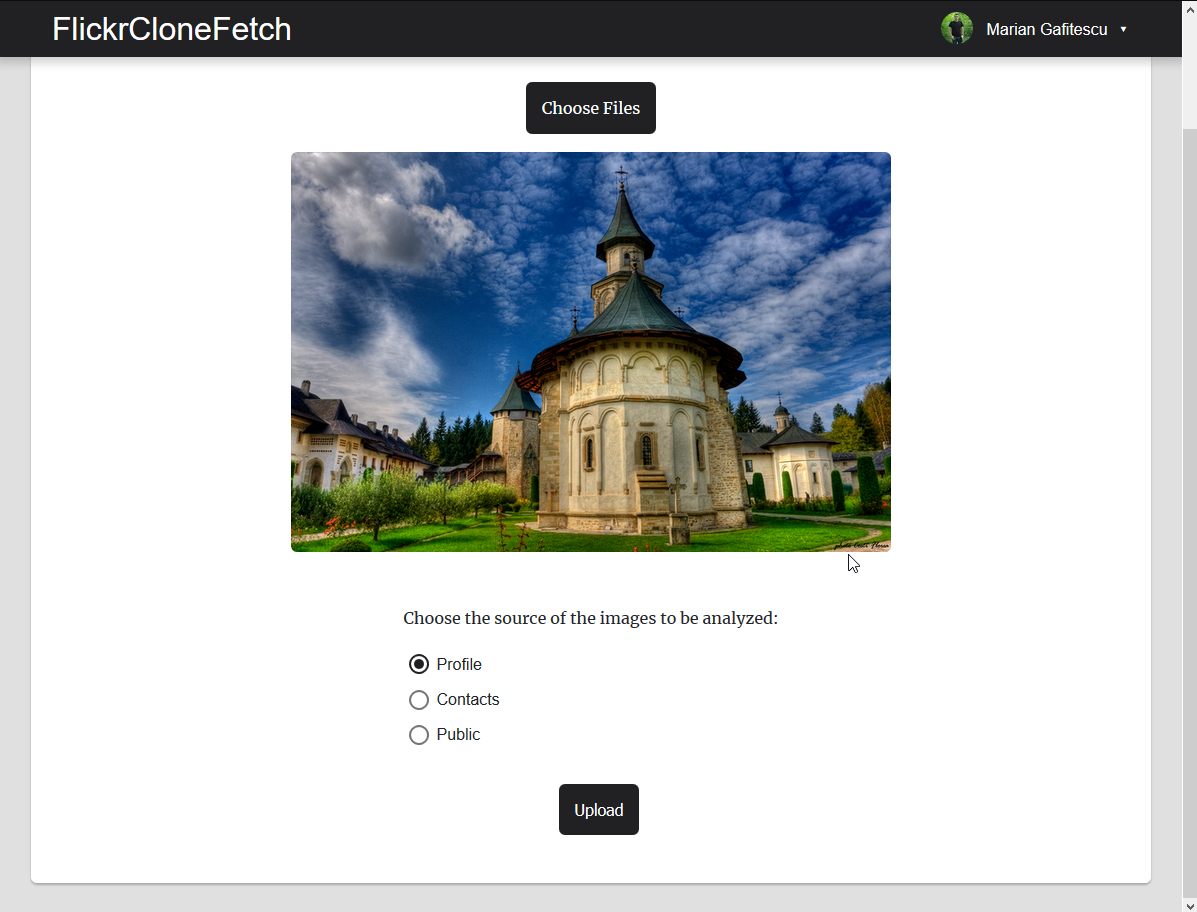
\includegraphics[width=1.0\textwidth]{images/preview.png}
        \caption{Vizualizarea imaginii alese }
    \end{center}
\end{figure}


\pagebreak
\subsection{Aplicația procesează cererea}
\begin{figure}[!htbp]
    \begin{center}
        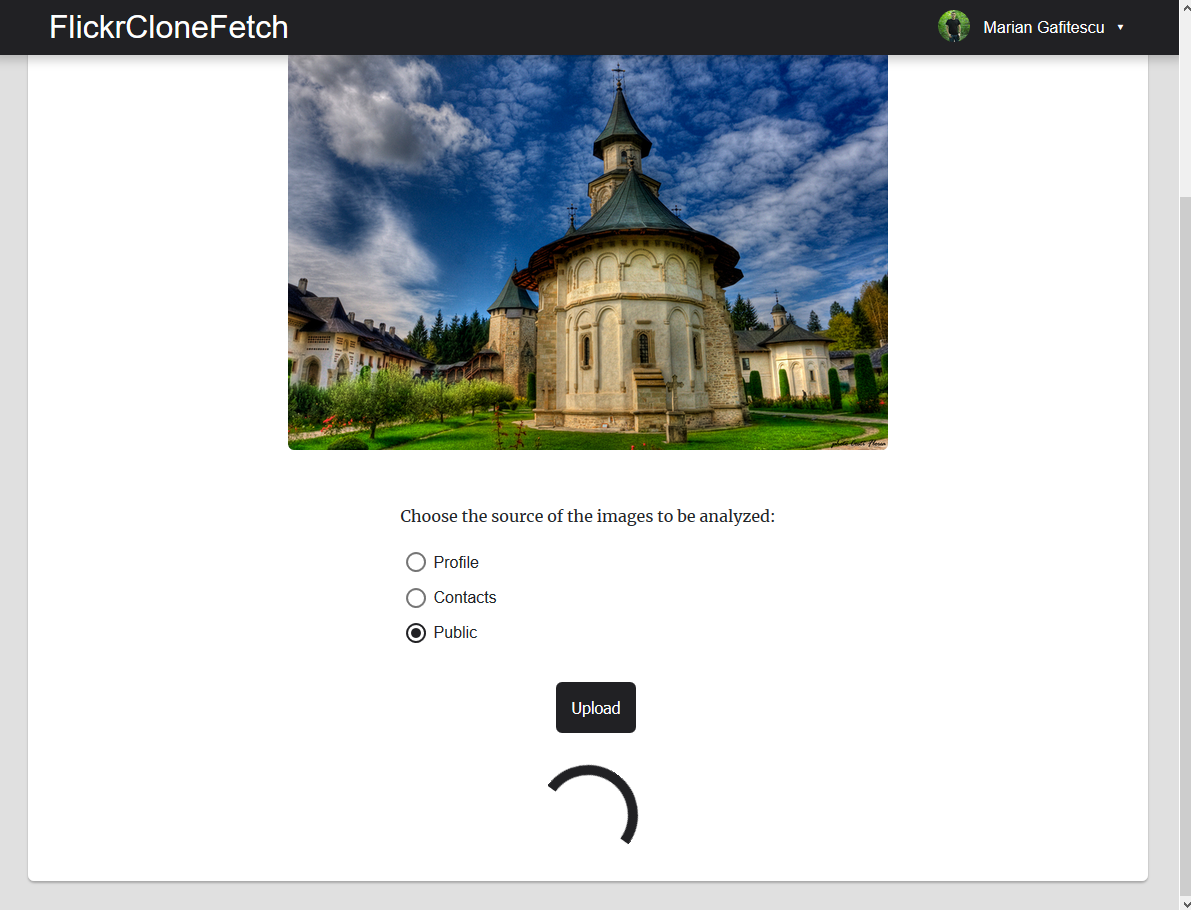
\includegraphics[width=1.0\textwidth]{images/loading.png}
        \caption{Procesarea cererii utilizatorului }
    \end{center}
\end{figure}

\pagebreak
\subsection{Aplicația afișează rezultatele corespunzătoare}
\begin{figure}[!htbp]
    \begin{center}
        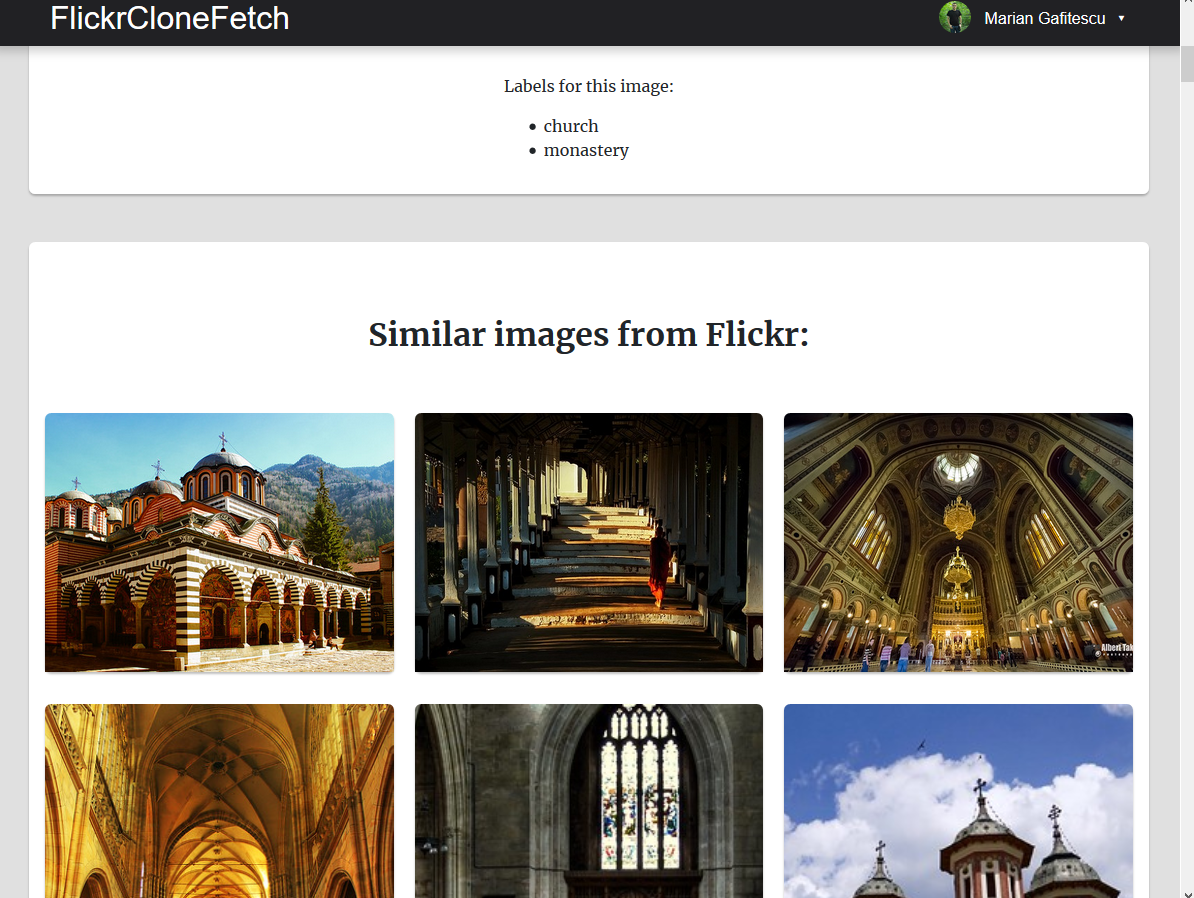
\includegraphics[width=1.0\textwidth]{images/results.png}
        \caption{Afișarea rezultatelor }
    \end{center}
\end{figure}